\documentclass[tikz,border=5pt]{standalone}
\usepackage{fontspec}
\setmainfont{Times New Roman}
\usepackage{unicode-math}
\setmathfont{Cambria Math}
\usetikzlibrary{shapes.geometric,positioning,fit,backgrounds,arrows.meta,calc}

\begin{document}
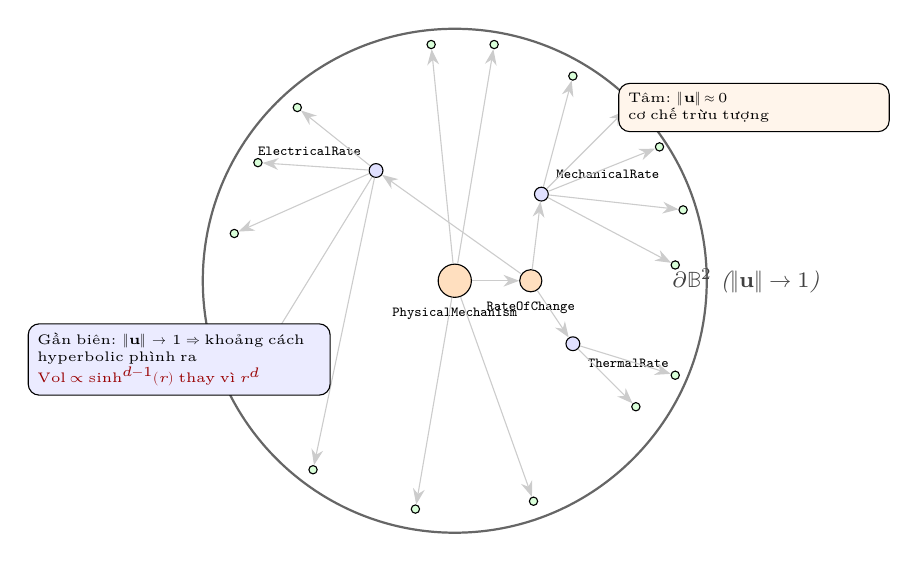
\begin{tikzpicture}[
  nd/.style={circle, draw, inner sep=1.2pt, minimum size=5pt},
  root/.style={nd, fill=orange!25, minimum size=8pt},
  mid/.style={nd, fill=blue!12, minimum size=4pt},
  leaf/.style={nd, fill=green!15, minimum size=3pt, inner sep=0.5pt},
  arrow/.style={-{Stealth[length=2mm]}, thin, gray!40},
  label/.style={font=\scriptsize\itshape, text=gray!60!black},
]

% ====== Disk boundary ======
\draw[thick, black!60] (0,0) circle (3.2);
\node[font=\footnotesize\itshape, text=gray!50!black] at (3.7, 0) {$\partial\mathbb{B}^2$ ($\|\mathbf{u}\|\to1$)};

% ====== Root mechanisms (center) ======
\node[root, inner sep=3pt, minimum size=12pt] (root1) at (0,0) {};
\node[font=\tiny, below=0pt of root1] {\texttt{PhysicalMechanism}};
\node[root, right=0.6cm of root1, inner sep=2pt, minimum size=8pt] (root2) {};
\node[font=\tiny, below=0pt of root2] {\texttt{RateOfChange}};

\draw[arrow] (root1) -- (root2);

% ====== Mid-level nodes ======
\node[mid, minimum size=5pt] (mid1) at (1.1, 1.1) {};
\node[font=\tiny, above right=0pt of mid1] {\texttt{MechanicalRate}};
\node[mid, minimum size=5pt] (mid2) at (-1.0, 1.4) {};
\node[font=\tiny, above left=0pt of mid2] {\texttt{ElectricalRate}};
\node[mid, minimum size=5pt] (mid3) at (1.5, -0.8) {};
\node[font=\tiny, below right=0pt of mid3] {\texttt{ThermalRate}};

\draw[arrow] (root2) -- (mid1);
\draw[arrow] (root2) -- (mid2);
\draw[arrow] (root2) -- (mid3);

% ====== Leaf nodes near boundary ======
\node[leaf, minimum size=3pt] (l1) at (2.6, 1.7) {};
\node[leaf, minimum size=3pt] (l2) at (2.9, 0.9) {};
\node[leaf, minimum size=3pt] (l3) at (2.2, 2.2) {};
\node[leaf, minimum size=3pt] (l4) at (2.8, 0.2) {};
\node[leaf, minimum size=3pt] (l5) at (1.5, 2.6) {};
\node[leaf, minimum size=3pt] (l6) at (2.3, -1.6) {};
\node[leaf, minimum size=3pt] (l7) at (2.8, -1.2) {};
\node[leaf, minimum size=3pt] (l8) at (-2.5, 1.5) {};
\node[leaf, minimum size=3pt] (l9) at (-2.8, 0.6) {};
\node[leaf, minimum size=3pt] (l10) at (-2.0, 2.2) {};
\node[leaf, minimum size=3pt] (l11) at (-2.6, -1.2) {};
\node[leaf, minimum size=3pt] (l12) at (-1.8, -2.4) {};
\node[leaf, minimum size=3pt] (l13) at (0.5, 3.0) {};
\node[leaf, minimum size=3pt] (l14) at (-0.3, 3.0) {};
\node[leaf, minimum size=3pt] (l15) at (1.0, -2.8) {};
\node[leaf, minimum size=3pt] (l16) at (-0.5, -2.9) {};

\draw[arrow] (mid1) -- (l1);
\draw[arrow] (mid1) -- (l2);
\draw[arrow] (mid1) -- (l3);
\draw[arrow] (mid1) -- (l4);
\draw[arrow] (mid1) -- (l5);
\draw[arrow] (mid3) -- (l6);
\draw[arrow] (mid3) -- (l7);
\draw[arrow] (mid2) -- (l8);
\draw[arrow] (mid2) -- (l9);
\draw[arrow] (mid2) -- (l10);
\draw[arrow] (mid2) -- (l11);
\draw[arrow] (mid2) -- (l12);
\draw[arrow] (root1) -- (l13);
\draw[arrow] (root1) -- (l14);
\draw[arrow] (root1) -- (l15);
\draw[arrow] (root1) -- (l16);

% ====== Annotation: exponential room ======
\node[draw, rounded corners, fill=blue!8, align=left, font=\tiny, text width=3.6cm]
  (ann) at (-3.5, -1.0)
  {Gần biên: $\|\mathbf{u}\|\to1$ $\Rightarrow$ khoảng cách hyperbolic phình ra\\
   \textcolor{red!60!black}{$\mathrm{Vol}\propto\sinh^{d-1}(r)$ thay vì $r^d$}};

% ====== Center annotation ======
\node[draw, rounded corners, fill=orange!8, align=left, font=\tiny, text width=3.2cm]
  at (3.8, 2.2)
  {Tâm: $\|\mathbf{u}\|\approx0$\\ cơ chế trừu tượng};

\end{tikzpicture}
\end{document}